%%%%%%%%%%%%%%%%%%%%%%%%%%%%%%%%%%%%%%%%%%%%%%%%%%%%%%%%%%%%%%%%%%%%%%
%%%%%%%%%%%%%%%%%%%%%%%%%%%%%%%%%%%%%%%%%%%%%%%%%%%%%%%%%%%%%%%%%%%%%%
%%%%%%%%%%%%%%%%%%%%%%%%%%%%%%%%%%%%%%%%%%%%%%%%%%%%%%%%%%%%%%%%
%   kmake afb_sig-ps
\documentclass[12pt]{article}


%%%%%%%%%%%%%%%%%%%%%%%%%%%%%%%%%%%%%%%%%%%%%%%%%%%%%%%%%%%%%%%%%
\usepackage{epsfig}

\usepackage{amsmath}
\usepackage{amssymb}
\usepackage{euscript}

\usepackage{fancybox}
\usepackage{xcolor}


%%%%%%%%%%%%%%%%%%%%%%%%%%%%%%%%%%%%%%%%%%%%%%%%%%%%
\input Energy.tex
%\def\Energy{MZ-1.8GeV (had.)}
\def\Angle{$\theta^{\bullet}$}


%%%%%%%%%%%%%%%%%%%%%%%%%%%%%%%%%%%%%%%%%%%%%%%%%%%%%%%%%%%%%%%
%  copied from seminar.con
\def\titbox#1{\begin{center}\doublebox{#1}\end{center}}

\newcommand{\KK}{${\cal KK}$}
\def\OrderLL#1{${\cal O}(#1)_{\rm LL}$}


%%%%%%%%%%%%%%%%%%%%%%%%%%%%%%%%%%%%%%%%%%%%%%%%%%%%%%%%%%%%%%%
\textwidth  = 16cm % <-- maximum CERN
\textheight = 22cm % <-- maximum CERN
\hoffset    = -1cm
\voffset    = -1cm


%%%%%%%%%%%%%%%%%%%%%%%%%%%%%%%%%%%%%%%%%%%%%%%%%%%%%%%
%%%%%%%%%%%%%%%%%%%%%%%%%%%%%%%%%%%%%%%%%%%%%%%%%%%%%%%
\begin{document}                     %%%%%%%%%%%%%%%%%%


%//////////////////////////////////////////////////////////////////////////////////
%//////////////////////////////////////////////////////////////////////////////////
%//////////////////////////////////////////////////////////////////////////////////

\titbox{{\bf\color{red} CEEX $\sigma$ and $A_{\rm FB}$, energy cut-off study }}

\vspace{10mm}
\begin{center}
\epsfig{file=afb_int-tab1.eps,width=170mm}
\end{center}

\large
Process: $e^-e^+ \to f\bar{f}$, $f=\mu^-$, at \Energy.
Energy cut: $v<v_{\max}$, where $v=1-M^2_{f\bar{f}}/s$.
Scattering angle for $A_{\rm FB}$ is $\theta=$\Angle.
No cut in \Angle. 
E-W corr. in \KK\  according to DIZET 6.x.
\OrderLL{\alpha^3} EEX3 matrix element in \KK\ (without ISR*FSR interf.)
\KK{}sem is semianalytical part of \KK.
(Angle $\theta^{\bullet}$ is from Phys. Rev. {\bf D41}, 1425 (1990).)

%-----------------------------------------------------------
\vfill


%//////////////////////////////////////////////////////////////////////////////////
%//////////////////////////////////////////////////////////////////////////////////
%//////////////////////////////////////////////////////////////////////////////////
\newpage
\titbox{{\large\bf\color{magenta} Total cross section $\sigma$, energy cut-off stydy}}

\begin{center}
\epsfig{file=afb_int-Gsig.eps,width=160mm}
\end{center}

The same as in the table.
The {\color{red} ISR$\otimes$FSR  interf.} switched on/off wherever possible.
No cut in \Angle.
Reference $\sigma_{\rm ref}$ = semianalytical of \KK{}sem,
(no ISR$\otimes$FSR,  up to \OrderLL{\alpha^3}, JSW exponentiation).
EEX2 data points from KORALZ/YFS3 version 4.03 
(QED up to \OrderLL{\alpha^2}, ISR$\otimes$FSR off).
%-----------------------------------------------------------
\vfill



%//////////////////////////////////////////////////////////////////////////////////
%//////////////////////////////////////////////////////////////////////////////////
%//////////////////////////////////////////////////////////////////////////////////
\newpage
\titbox{{\large\bf\color{magenta} Charge asymmetry $A_{\rm FB}$, energy cut-off study}}

\begin{center}
\epsfig{file=afb_int-Gafb.eps,width=160mm}
\end{center}

The same as in the table.
The {\color{red} ISR$\otimes$FSR  interf.} switched on/off wherever possible.
No cut in \Angle.
Reference $A_{\rm FB}^{\rm ref}$ =  semianalytical \KK{}sem,
(no ISR$\otimes$FSR,  up to \OrderLL{\alpha^3}, JSW exponentiation).
EEX2 data points are from KORALZ/YFS3 version 4.03 
(QED up to \OrderLL{\alpha^2}, ISR$\otimes$FSR off.).
%-----------------------------------------------------------
\vfill



%//////////////////////////////////////////////////////////////////////////////////
%//////////////////////////////////////////////////////////////////////////////////
%//////////////////////////////////////////////////////////////////////////////////
\newpage
\titbox{{\large\bf\color{magenta} Total x-section $\sigma$, comparison with Zfitter}}

\begin{center}
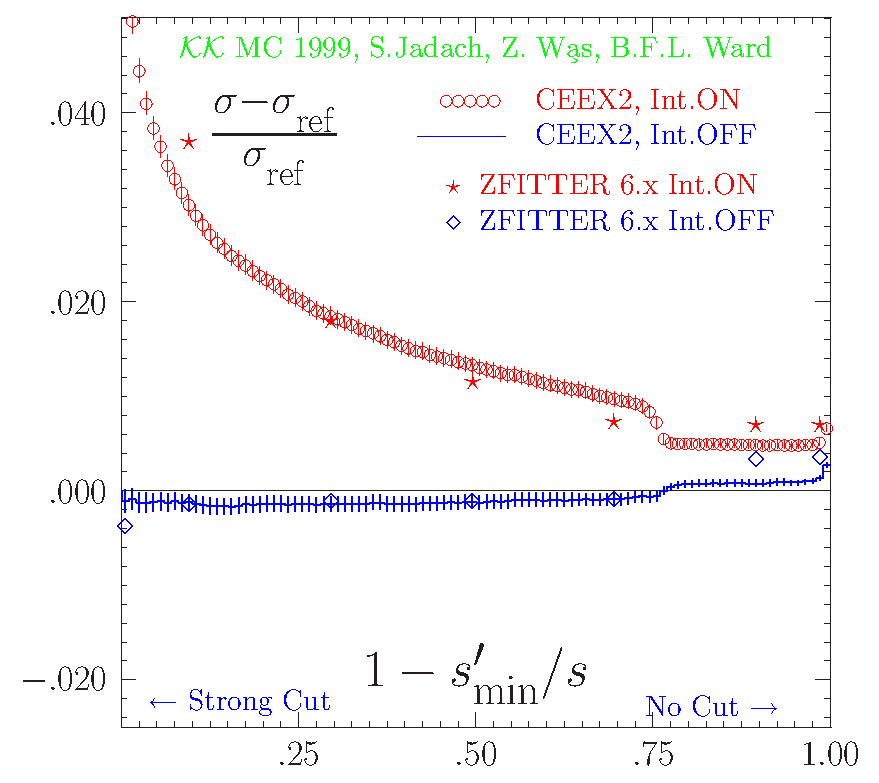
\epsfig{file=afb-int-GsigZFtheta1.eps,width=160mm}
\end{center}

Comparison with Zfitter 6.xx.
The {\color{red} ISR$\otimes$FSR  interf.} switched on/off.
No cut in $\theta_1$.
Reference $\sigma_{\rm ref}$ = semianalytical of \KK{}sem,
(no ISR$\otimes$FSR,  up to \OrderLL{\alpha^3}, JSW exponentiation).

\vfill
%-----------------------------------------------------------


%//////////////////////////////////////////////////////////////////////////////////
%//////////////////////////////////////////////////////////////////////////////////
%//////////////////////////////////////////////////////////////////////////////////
\newpage
\titbox{{\large\bf\color{magenta} Charge asymmetry $A_{\rm FB}$, comparison with Zfitter}}

\begin{center}
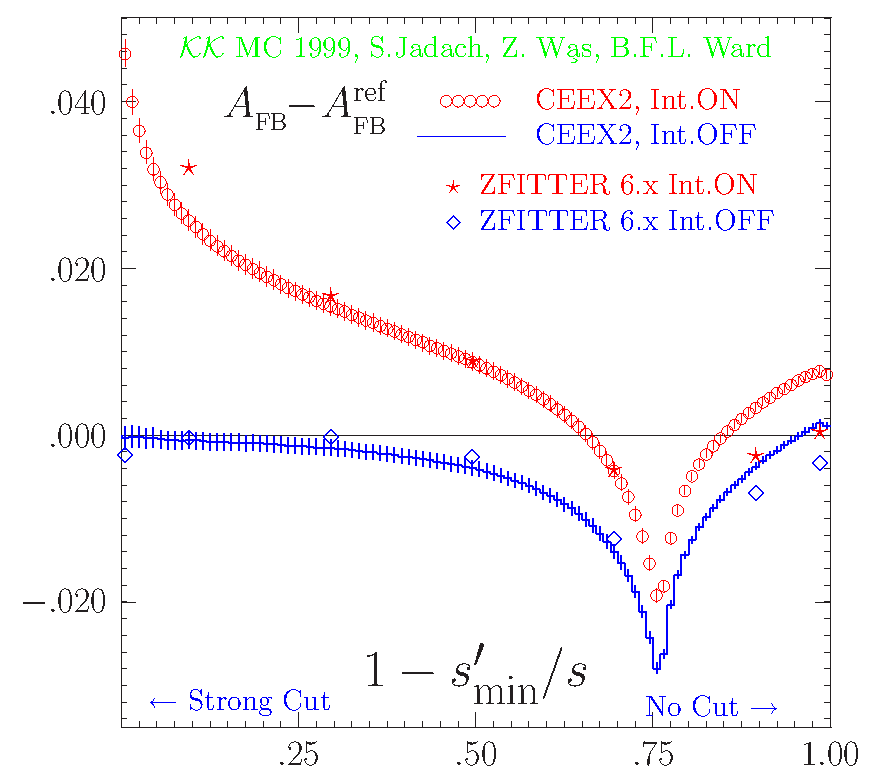
\epsfig{file=afb-int-GafbZFtheta1.eps,width=160mm}
\end{center}

Comparison with Zfitter 6.xx.
The {\color{red} ISR$\otimes$FSR  interf.} switched on/off.
No cut in $\theta_1$.
Reference $A_{\rm FB}^{\rm ref}$ =  semianalytical \KK{}sem,
(no ISR$\otimes$FSR,  up to \OrderLL{\alpha^3}, JSW exponentiation).

%-----------------------------------------------------------
\vfill



%//////////////////////////////////////////////////////////////////////////////////
%//////////////////////////////////////////////////////////////////////////////////
%//////////////////////////////////////////////////////////////////////////////////
\newpage
\titbox{{\large\bf\color{magenta} 
                      Physical Precision of CEEX, NEW!!! }}

%-----------------------------------------------------------
\begin{center}
\epsfig{file=afb_int-sigHO.eps,width=100mm}\\
\epsfig{file=afb_int-afbHO.eps,width=100mm}
\end{center}

The difference between second and first order CEEX results for at \Energy.
The energy cut is on $s'/s$, where $s'=m^2_{f\bar{f}}$.

{\color{blue} Scattering angle is $\theta=$\Angle. }
{\color{blue}\small  [Angle $\theta^{\bullet}$ is defined in Phys. Rev. {\bf D41}, 1425 (1990)]}

%-----------------------------------------------------------
\vfill



\end{document}                       %%%%%%%%%%%%%%%%%%
%%%%%%%%%%%%%%%%%%%%%%%%%%%%%%%%%%%%%%%%%%%%%%%%%%%%%%%
%%%%%%%%%%%%%%%%%%%%%%%%%%%%%%%%%%%%%%%%%%%%%%%%%%%%%%%


